\documentclass[Royal,times,sageh]{sagej}

\usepackage{moreverb,url,natbib, multirow, tabularx}
\usepackage[colorlinks,bookmarksopen,bookmarksnumbered,citecolor=red,urlcolor=red]{hyperref}



% tightlist command for lists without linebreak
\providecommand{\tightlist}{%
  \setlength{\itemsep}{0pt}\setlength{\parskip}{0pt}}



\usepackage{booktabs}
\usepackage{longtable}
\usepackage{array}
\usepackage{multirow}
\usepackage{wrapfig}
\usepackage{float}
\usepackage{colortbl}
\usepackage{pdflscape}
\usepackage{tabu}
\usepackage{threeparttable}
\usepackage{threeparttablex}
\usepackage[normalem]{ulem}
\usepackage{makecell}
\usepackage{xcolor}


\begin{document}


\setcitestyle{aysep={,}}

\title{TTS2016R: A dataset to study population and employment patterns
from the 2016 Transportation Tomorrow Survey (TTS) in the Greater
Toronto and Hamilton Area, Canada}

\runninghead{}

\author{Anastasia Soukhov\affilnum{}, Antonio Páez\affilnum{}}

\affiliation{\affilnum{}{}}



\begin{abstract}
This paper describes and visualises the data contained within the
\{TTS2016R\} data-package created in \texttt{R}, the statistical
computing and graphics language. In addition to a synthetic example,
\{TTS2016R\} contains home-to-work commute information for the Greater
Golden Horseshoe area in Canada retrieved from the 2016 Transportation
Tomorrow Survey (TTS). Included are all Traffic Analysis Zones (TAZ),
the number of people who are employed full-time per TAZ, the number of
jobs per TAZ, origin-destination trips, and calculated car travel time
from TAZ origin-destination centroid pairs. To illustrate how this
information can be analysed to understand patterns in commuting, we
estimate a distance-decay curve (i.e., impedance function) for the
region. \{TTS2016R\} can be freely downloaded and explored at:
\url{https://github.com/soukhova/TTS2016R} where the documentation and
code involved in data creation, manipulation, and the final data
products are detailed.
\end{abstract}

\keywords{Jobs; population; travel time; impedance; Greater Toronto and
Hamilton Area; Ontario, Canada; R}

\maketitle

\hypertarget{introduction}{%
\section{Introduction}\label{introduction}}

This manuscript presents the open data product
\href{https://github.com/soukhova/TTS2016R}{\{TTS2016R\}}. Open data
products are the result of turning source data (open or otherwise) into
accessible information that adds value to the original inputs
\citep[see][]{Arribas2021open}. The product presented in this paper is
an \texttt{R} data package which currently consists of three objects
which are sourced from the 2016 Transportation Tomorrow Survey (TTS) or
are curated to facilitate the use and analysis of TTS data. This package
includes person-to-jobs origin-destinations, traffic analysis zone (TAZ)
boundaries, and planning/municipality boundaries for the Greater Golden
Horse area (GGH) located in southern Ontario, Canada
\citep{data_management_group_tts_2018}. In addition, the package
includes TAZ centroid-to-centroid travel times by car computed using
package \{r5r\} \citep{Pereira2021r5r}. The aim of this paper is to walk
readers through the empirical home-based work commute data set,
illustrate the calculation of an impedance function that can be used to
calculate accessibility to employment, and invite its use in other
applications.

\hypertarget{home-to-work-commute-data}{%
\section{Home-to-work commute data}\label{home-to-work-commute-data}}

\{TTS2016R\} includes counts of fully-employed population by place of
residence (origin) and counts of full-time jobs by place of work
(destination) aggregated by TAZ (n=3,764 within the survey boundaries).
TAZ typically are defined based on land-use and population demographics
in order to estimate the number of trips produced and attracted to each
zone \citep{meyer_urban_2001}. As such, each TAZ is uniquely identified
using the GTA06 Zoning System which can be used to join to the
origin-destination table (i.e., trips taken).

The number of jobs (3,081,885) and workers (3,446,957) in this package
are organized in the form of an origin-destination table which is
indicative of home-to-work commute patterns (there are 3,446,957
potential interactions). These data were retrieved from the TTS Data
Retrieval System on October 28, 2021 and reflect the potential
interaction of full-time employed people and jobs within the GGH survey
boundaries shown in Figure \ref{fig:TTS-16-survey-area} as defined by
the 2016 TTS methodology \citep{data_management_group_tts_2018}.

Also included in \{TTS2016R\} are travel times and cost of travel from
origin to destination by car; travel times are calculated using the
\texttt{R} package \{r5r\}. These travel times are useful to estimate
the cost of travel and to calculate impedance functions, among other
possible applications. For simplicity, all interactions within
\{TTS2016R\} are assumed to be taken by car, and the travel time is
calculated from an origin TAZ centroid to a destination TAZ centroid.
The centroid is snapped to the nearest street line by \texttt{r5r} and
the travel time is calculated for all trips assuming a car travel mode.
Additionally, only travel times less than or equal to 180 mins (3 hrs)
are calculated; this threshold represents 99\% of trip's travel times
which are summarized in Figure \ref{fig:TTS-16-survey-area}.

\begin{figure}

{\centering 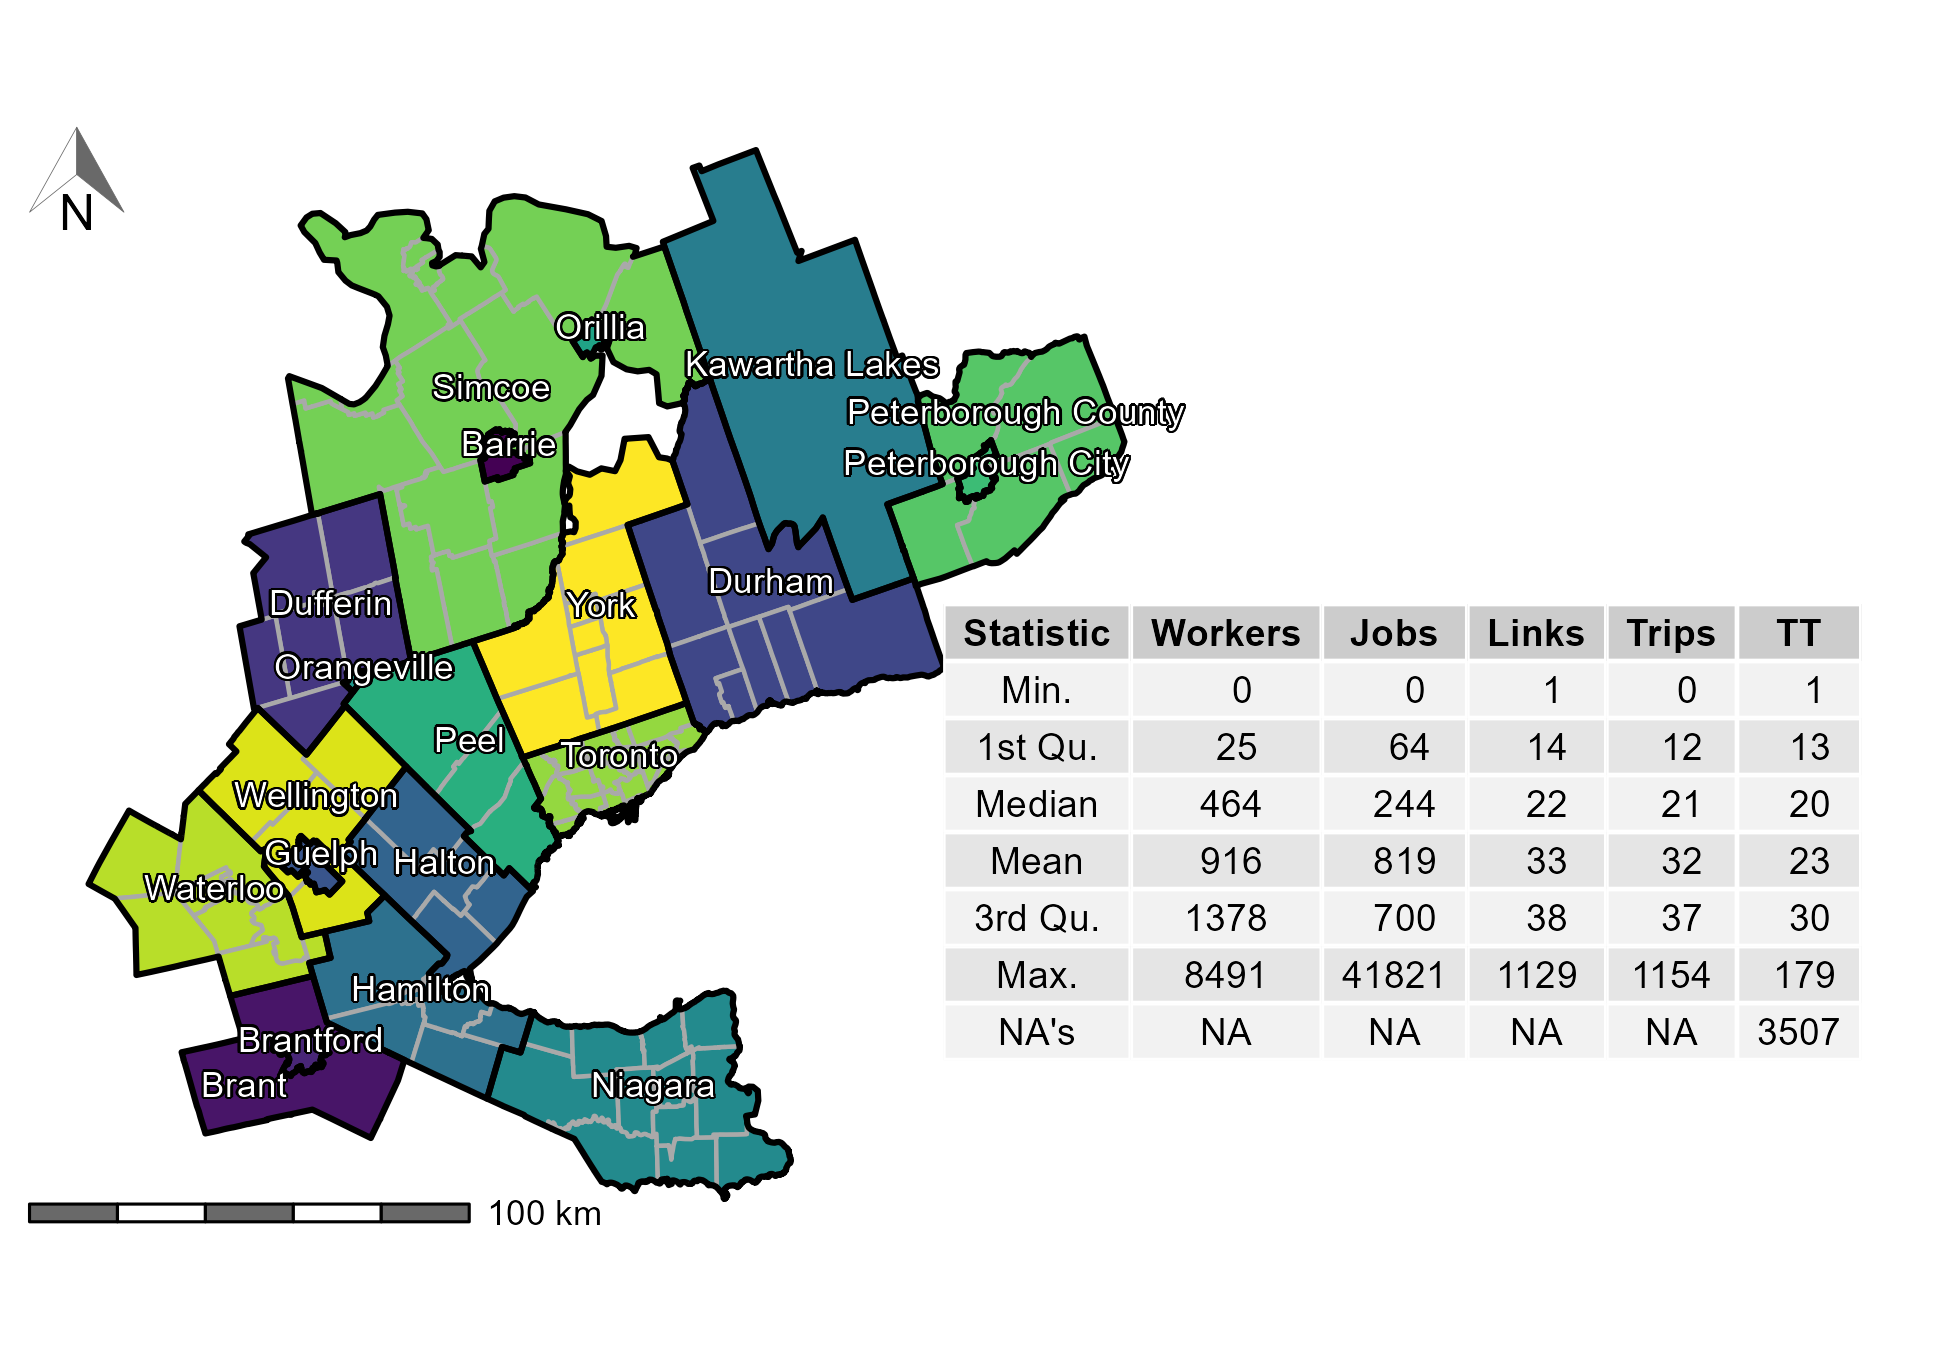
\includegraphics[width=1\linewidth]{images/TTS16-survey-area} 

}

\caption{\label{fig:TTS-16-survey-area}TTS 2016 study area within the GGH in Ontario, Canada along with the descriptive statistics of the trips, calculated origin-destination car travel time (TT), workers per TAZ, and jobs per TAZ. Contains 20 regions (black boundaries) and sub-regions (dark gray boundaries).}\label{fig:TTS-16-survey-area}
\end{figure}

\hypertarget{employed-individuals-and-jobs}{%
\subsection{Employed individuals and
jobs}\label{employed-individuals-and-jobs}}

The origin-destination table (i.e., trips) consists of a
cross-tabulation of people who are employed full-time by place of GGH
residence (origin) and places of GGH employment (destination) using the
GTA06 TAZ zoning system. It is important to note that the total number
of workers and jobs is the TTS 2016 region are not equal but the number
of trips taken are equal to the number of workers. Since the outer
boundaries of the TTS are permeable, workers who reside within the
boundaries but travel outside of the boundaries are counted as workers
within an origin TAZ, while jobs in TAZ that are filled by workers who
reside outside the GGH boundaries are \emph{unknown} since they were not
surveyed. This mismatch results in the total number of workers being
1.12 times larger than the number of jobs (i.e., 3,446,957 workers to
3,081,885 jobs). As such, the origin-destination table contained in
\{TTS2016R\} offers a perspective on all workers in the GGH and their
home-based trips to places of GGH employment.

\begin{figure}
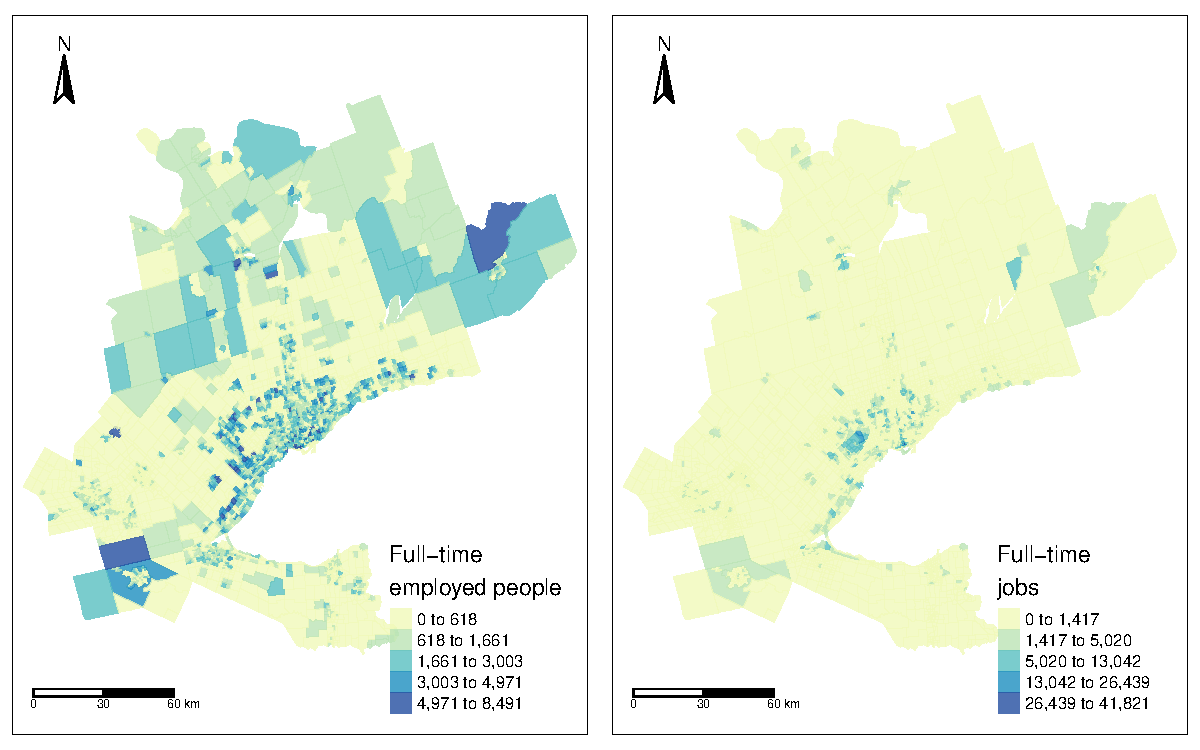
\includegraphics[width=1\linewidth]{Manuscript-Data-Package_files/figure-latex/tts-workers-jobs-plot-1} \caption{\label{fig:tts-workers-jobs-plot}Number of workers (left) and jobs (right) in each TAZ in the 2016 TTS.}\label{fig:tts-workers-jobs-plot}
\end{figure}

Figure \ref{fig:tts-workers-jobs-plot} presents the number of workers
and jobs per TAZ. It can be observed that the spatial distribution of
jobs and workers is unequal, which is indicative of a jobs-housing
imbalance that can impact accessibility in a region
\citep{Levine1998rethinking}. It can also be seen that there is a higher
number of TAZ with no workers than zones with no jobs (i.e., 791 TAZ
with no workers : 396 TAZ with no jobs) and the mean of workers per TAZ
is higher than the mean of jobs (i.e., 916 workers : 819 jobs) the
number TAZ with an extreme number of jobs at the highest and lowest
percentiles is significantly higher than the number of workers.

\hypertarget{calculated-travel-time}{%
\subsection{Calculated travel time}\label{calculated-travel-time}}

As mentioned, \{TTS2016R\} also includes travel time data for each
home-to-work trip as displayed in Figure \ref{fig:plot-tt-ttpertrip}.
This travel time corresponds to a car commute calculated using the R
package \{r5r\} (see descriptive statistics in Figure
\ref{fig:TTS-16-survey-area}). It is important to note that travel times
within this data set are calculated assuming only car travel and one
departure time for all origins. These assumptions are not completely
realistic since we know a small proportion of trips are taken by non-car
modes and travel time departures varies. However, it is not possible
from the data retrieval system to obtain higher order tabulations so we
carry on with the assume that all trips are taken by one-time departure
car trip.

\begin{figure}
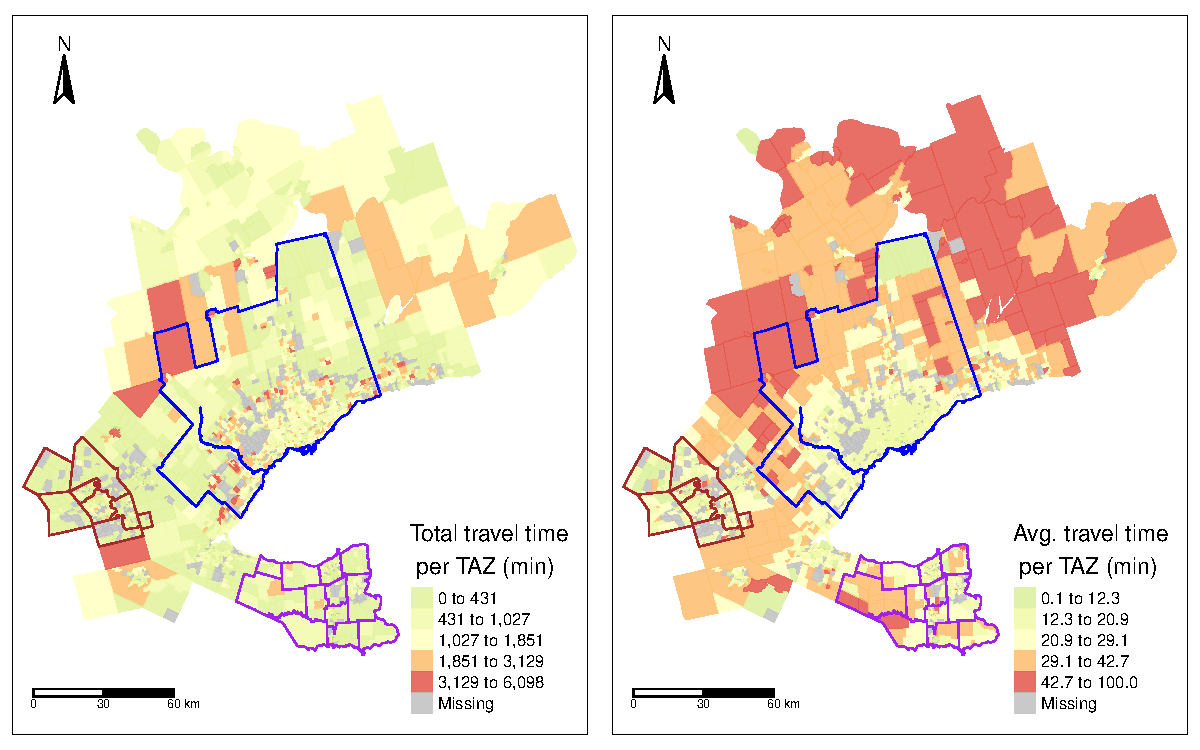
\includegraphics[width=1\linewidth]{Manuscript-Data-Package_files/figure-latex/plot-tt-ttpertrip-1} \caption{\label{fig:plot-tt-ttpertrip}Calculated total worker travel time (left) and average worker travel time (right) for each TAZ in the 2016 TTS.}\label{fig:plot-tt-ttpertrip}
\end{figure}

\newpage

As can be observed in Figure \ref{fig:plot-tt-ttpertrip}, the total
travel time resembles the spatial trend distribution in the number of
employed people in the previous plot (Figure
\ref{fig:tts-workers-jobs-plot}) and the spatial distribution of the
average travel time is distinct from other plots presented so far. We
can see that in areas around the south-eastern border that make up the
Greater Toronto and Hamilton Area (GTHA), Niagara and Waterloo, the
average travel times are moderately low. Further from these areas,
travel times are higher. Interestingly, even in eastern areas (e.g.,
Peterborough) with high employment and high job concentration, average
travel time is higher than within the GTHA.

\hypertarget{calibrating-an-impedance-function}{%
\subsection{Calibrating an impedance
function}\label{calibrating-an-impedance-function}}

Impedance functions are useful to understand mobility behaviour and are
used to estimate gravity models of spatial interaction
\citep{wilson1971, haynes_gravity_1985} and applied in accessibility
analysis
\citep{hansen_how_1959, talen_assessing_1998, paez_jobs_2013, barboza_balancing_2021}.
An impedance function \(f(\cdot)\) depends on the cost of travel
\(c_{ij}\) between locations \(i\) and \(j\) (all which is supplied in
the travel time and origin-destination table within \{TTS2016R\}).

A useful technique to calibrate an impedance function is to use the trip
length distribution (TLD) as measured from origin-destination data
\citep{horbachov_theoretical_2018, batista_estimation_2019}. The TLD is
the representation of the likelihood that a proportion of trips are
taken at a specific travel cost. In our data set, where we assume cost
is travel time, the impedance function maps low travel times to higher
proportions of trips, and high travel times are mapped to low proportion
of trips.

Using the data contained in \{TTS2016R\}, we fit the empirical TLD to a
density distribution using maximum likelihood techniques and the
Nelder-Mead method for direct optimization available within the
\texttt{R} package \{fitdistrplus\} \citep{fitdistrplus_2015}. Based on
goodness-of-fit criteria and diagnostics seen in Figure
\ref{fig:TLD-Gamma-plot}, the gamma distribution is selected. The
`shape' parameter is \(\alpha\) = 2.019, the estimated `rate' is
\(\beta\) = 0.094 , and \(\Gamma(\alpha)\) is defined in Equation
(\ref{gamma-dist}).

\begin{figure}

{\centering 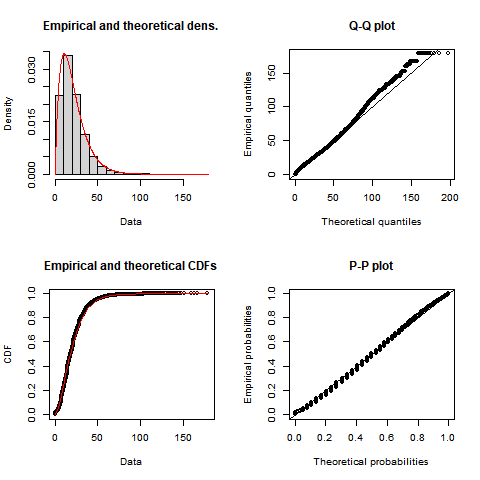
\includegraphics[width=0.75\linewidth]{images/impedance_function} 

}

\caption{\label{fig:TLD-Gamma-plot}Empirical TTS 2016 home-based car TLD (black) and calibrated gamma distribution impedance function (red) with associated Q-Q and P-P plots}\label{fig:TLD-Gamma-plot}
\end{figure}

\begin{equation}
\label{gamma-dist}
\begin{array}{l}\ 
f(x, \alpha, \beta) = \frac {x^{\alpha-1}e^{-\frac{x}{\beta}}}{ \beta^{\alpha}\Gamma(\alpha)} \quad \text{for } 0 \leq x \leq \infty\\
\Gamma(\alpha) =  \int_{0}^{\infty} x^{\alpha-1}e^{-x} \,dx\\
\end{array}
\end{equation}

\newpage

\hypertarget{concluding-remarks}{%
\section{Concluding remarks}\label{concluding-remarks}}

The open data product introduced in this paper shares tables for
home-to-work related data from the 2016 TTS. In addition, inter-centroid
travel time tables are calculated, and the planning/municipality
boundaries are included as a compliment. This open data product,
\{TTS2016R\}, is freely available to explore in an \texttt{R}
environment. One possible use of this data, as showcased in this paper,
is the calibration of impedance functions which in turn can be used for
accessibility analysis.

In the spirit of novel and original research, we hope readers value the
efforts made to detail the data in order to improve transparency in our
work and encourage others to replicate and, hopefully, inspire research
of their own. We see this product as providing open infrastructure for
additional TTS or complimentary data sets to be amended by the authors
or wider open-source community in the future.

\bibliographystyle{sageh}
\bibliography{bibfile}


\end{document}
